\documentclass{beamer}
\usetheme{Madrid}
\usecolortheme{default}

%\usepackage[T1]{fontenc}				% Output font encoding for international characters, renders WRONG on Windows
\usepackage{sansmathfonts}				% Sans Serif equations
\usepackage[utf8]{inputenc}				% Encoding of files: utf8
\renewcommand*\familydefault{\sfdefault} 		% Sans Serif as default font

\definecolor{BlueITBA}{HTML}{00558c} 
\colorlet{beamer@blendedblue}{BlueITBA}
\setbeamertemplate{caption}{\scriptsize\insertcaption}
\setbeamertemplate{itemize items}[circle]
%\setbeamertemplate{itemize subitem}[triangle]
\setbeamertemplate{itemize subitem}{\raisebox{0.2em}{\scalebox{0.65}{$\blacktriangleright$}}}   % Second level

%\setbeamertemplate{enumerate items}[default]
\setbeamertemplate{section in toc}{\inserttocsectionnumber.~\inserttocsection} 

\hypersetup{colorlinks,linkcolor=,urlcolor=blue}

% Setup the language and its properties (choose only one)
\usepackage[spanish, es-tabla, es-nodecimaldot]{babel}
\addto\captionsspanish{\renewcommand{\contentsname}{Contenido}}

\usepackage{graphicx}
%\usepackage{tikz}						% Required for title page
%\usepackage{bm}

\usepackage{ulem}
\usepackage{listings}
\usepackage{adjustbox}
\definecolor{vgreen}{RGB}{104,180,104}
\definecolor{vblue}{RGB}{49,49,255}
\definecolor{vorange}{RGB}{255,143,102}
\lstset{
	basicstyle=\scriptsize,
	language=Verilog,
	tabsize=2,
	keywordstyle=\color{vblue},
	identifierstyle=\color{black},
	commentstyle=\color{vgreen},
	showstringspaces=false
}

\title[HDL Coder]{MATLAB\texttrademark \space HDL Coder}
\subtitle{Introducción al Toolbox de MATLAB\texttrademark}
\author{Dr. Pablo \textsc{Cossutta}}
\institute[]{}
\date{Julio 2020}
\logo{
\includegraphics[height=1.5cm]{figs/logo_itba.png}} 
 
\begin{document}
\beamertemplatenavigationsymbolsempty % Disable Nav Bar
% Title and Intro
\maketitle
\logo{}

\renewcommand{\arraystretch}{1.3}

% 1
\begin{frame}{Necesidad}
	\begin{itemize}
		\item Verilog/VHDL son herramientas que simplifican el diseño de circuitos digitales
		\begin{itemize}
			\item No fueron pensadas para realizar algoritmos complejos
			\item La aritmética de Punto Fijo es complicada
			\begin{itemize}
				\item Ya que el usuario/programador debe corregir el punto acordemente en cada operación
			\end{itemize}
			\item La aritmética de Punto Flotante es costosa
			\begin{itemize}
				\item Utiliza una gran cantidad de recursos
				\item Alta latencia (generalmente 12 ciclos por operación)
			\end{itemize}
		\end{itemize}
		\item Existen diversas herramientas
		\begin{itemize}
			\item Librerias para utilizar en lenguajes HDL
			\begin{itemize}
				\item Sigue siendo necesario escribir código complejo
			\end{itemize}
			\item Matlab HDL Coder
			\begin{itemize}
				\item Independiente del fabricante de la FPGA
			\end{itemize}
			\item Herramientas específicas de cada fabricante
			\begin{itemize}
				\item Xilinx System Generator for DSPs
				\item DSP Builder for Intel\textsuperscript{\textregistered} FPGAs (Altera DSP Builder)
			\end{itemize}
		\end{itemize}
	\end{itemize}
\end{frame}

% 2
\begin{frame}{Restricciones}
\begin{itemize}
	\item Puede utilizarse tanto desde Matlab como desde Simulink
	\begin{itemize}
		\item Esta introducción está basada en Simulink
		\item Debido a que principalmente se utiliza en forma mixta con la simulación de los convertidores
		\item Permite integrar la lógica de control con la simulación del sistema
	\end{itemize}
	\item Utilización de Punto Fijo
	\begin{itemize}
		\item Punto Flotante se puede utilizar a expensas de una gran cantidad de recursos y latencia
	\end{itemize}
	\item Discrete Solver
	\begin{itemize}
		\item Fixed Step
	\end{itemize}
	\item Configuraciones complejas de Matlab
	\begin{itemize}
		\item HDL Workflow Advisor
		\begin{itemize}
			\item Algebraic Loops, Target Architecture, etc.
		\end{itemize}
	\end{itemize}
\end{itemize}
\end{frame}

% 3
\begin{frame}{Workflow Advisor}
\begin{figure}
	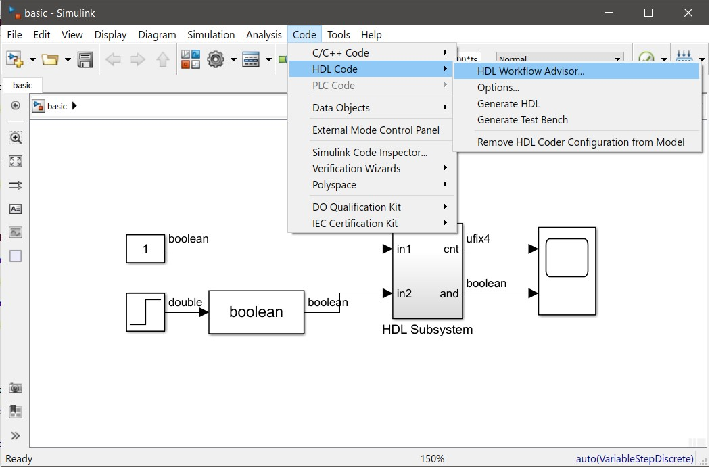
\includegraphics[page=1]{figs/figs.pdf}
\end{figure}
\end{frame}

% 4
\begin{frame}{HDL Coder Properties (1)}
\begin{itemize}
	\item Botón Derecho en HDL Subsystem, 
	\begin{itemize}
		\item HDL Code $\rightarrow$ HDL Coder Properties \ldots
	\end{itemize}
\end{itemize}
\vspace{-0.25em}
\begin{figure}
	\includegraphics[page=2, width=0.95\textwidth]{figs/figs.pdf}
\end{figure}
\end{frame}

% 5
\begin{frame}{HDL Coder Properties (2)}
\vspace{-0.25em}
\begin{figure}
	\includegraphics[page=3, width=0.9\textwidth]{figs/figs.pdf}
\end{figure}
\end{frame}

% 6
\begin{frame}{Ejemplo 1}
\begin{itemize}
	\item Modelo de simulación
\end{itemize}
\begin{figure}
	\includegraphics[page=4, width=0.75\textwidth]{figs/figs.pdf}%
\end{figure}
\begin{itemize}
	\item Detalle interno del bloque a sintetizar
\end{itemize}
\begin{figure}
	\includegraphics[page=5, width=0.85\textwidth]{figs/figs.pdf}%
\end{figure}
\end{frame}

% 7
\begin{frame}{Tipos de dato de Punto Fijo}
\begin{itemize}
	\item \texttt{ufixM\_En\_N}
	\begin{itemize}
		\item Tipo de dato no signado de $M$ bits en total con $N$ bits de parte fraccionaria 
		\item Rango: $\left[0, 2^{M-N}-2^{-N}\right]$ 
		\begin{itemize}
			\item Ej. \texttt{ufix8\_En2}: $\left[0, 2^{6}-2^{-2}\right] = \left[0, 63.75\right]$
		\end{itemize}
	\end{itemize}
	\item \texttt{sfix}
	\begin{itemize}
		\item Tipo de dato signado de $M$ bits en total con $N$ bits de parte fraccionaria 
		\item Rango: $\left[-2^{M-N-1}, 2^{M-N-1}-2^{-N}\right]$ 
		\begin{itemize}
			\item Ej. \texttt{sfix8\_En2}: $\left[-2^5, 2^5-2^{-2}\right] = \left[-32, 31.75\right]$
		\end{itemize}
	\end{itemize}
	\item Existen varios tipos predefinidos
	\begin{itemize}
		\item Por ej. \texttt{uint8}, \texttt{int8}
	\end{itemize}
	\item No es la única forma de definir un tipo de datos en punto fijo
	\begin{itemize}
		\item Por ej. \textit{Slope and Bias}
	\end{itemize}
\end{itemize}
\end{frame}

% 8
\begin{frame}[fragile]{Ejemplo 1 - Código generado (1)}
\begin{itemize}
	\item Se muestran solo las partes relevantes del código
	\item Entradas y salidas denominadas de la misma forma que en Simulink
	\begin{itemize}
		\item El diseño HDL que lo utilice solo debe instanciarlo
	\end{itemize}
	\item Utiliza \textit{enables} 
	\begin{itemize}
		\item Permite realizar fácilmente diversos \textit{sample time}
	\end{itemize}
\end{itemize}
\begin{columns}
\column{0.1\textwidth}
\column{0.4\textwidth}
	\begin{itemize}
		\item En el \texttt{top.v}
	\end{itemize}
\begin{center}\begin{adjustbox}{padding=2pt 0pt 0pt 0pt, cfbox=blue!50 1pt}\begin{lstlisting}[basicstyle=\tiny]
HDL_Subsystem HDL_Subsystem_inst(
	.clk(clk),
	.reset(rst_n),
	.clk_enable(en),
	.in1(j13),
	.in2(j14),
    .ce_out(),
    .cnt(cnt),
    .and_rsvd(j19));
\end{lstlisting}\end{adjustbox}\end{center}
\column{0.4\textwidth}
\begin{center}\begin{adjustbox}{padding=2pt 0pt 0pt 0pt, cfbox=blue!50 1pt}\begin{lstlisting}[basicstyle=\tiny]
module HDL_Subsystem
          (clk,
           reset,
           clk_enable,
           in1,
           in2,
           ce_out,
           cnt,
           and_rsvd);

  input   clk;
  input   reset;
  input   clk_enable;
  input   in1;
  input   in2;
  output  ce_out;
  output  [3:0] cnt;  // ufix4
  output  and_rsvd;
\end{lstlisting}\end{adjustbox}\end{center}
\column{0.1\textwidth}
\end{columns}
\end{frame}

% 9
\begin{frame}[fragile]{Ejemplo 1 - Código generado (2)}
\begin{itemize}
	\item La frecuencia de \texttt{ce\_out} es la del modelo 
	\begin{itemize}
		\item Permite conectar en cascada diversos subsistemas
	\end{itemize}
\end{itemize}
\begin{center}\begin{adjustbox}{padding=2pt 0pt 0pt 0pt, cfbox=blue!50 1pt}\begin{lstlisting}[basicstyle=\tiny]
  wire enb; 
  reg [3:0] Counter_Free_Running_out1;  // ufix4
  wire Logical_Operator_out1;
  assign enb = clk_enable; // Free running, Unsigned Counter
  //  initial value   = 0
  //  step value      = 1
  always @(posedge clk)
    begin : Counter_Free_Running_process
      if (reset == 1'b0) begin
        Counter_Free_Running_out1 <= 4'b0000;
      end
      else begin
        if (enb) begin
          Counter_Free_Running_out1 <= Counter_Free_Running_out1 + 4'b0001;
        end
      end
    end

  assign cnt = Counter_Free_Running_out1;
  assign Logical_Operator_out1 = in1 & in2;
  assign and_rsvd = Logical_Operator_out1;
  assign ce_out = clk_enable;
endmodule  // HDL_Subsystem
\end{lstlisting}\end{adjustbox}\end{center}
\end{frame}

% 10
\begin{frame}{Características}
\begin{columns}
\column{0.49\textwidth}
\begin{itemize}
	\item Configuración del Reset
	\begin{itemize}
		\item Sincrónicos vs Asincrónico
	\end{itemize}
	\item Oversampling
	\item Optimization
	\begin{itemize}
		\item Resource Sharing
		\item Flatten Hierarchy
		\item Sharing/Streaming Factor 
		\item Muchas mas
	\end{itemize}
	\item Las optimizaciones pueden ser
	\begin{itemize}
		\item Por Bloque
		\item Por Diseño
	\end{itemize}
\end{itemize}
\column{0.49\textwidth}
\begin{figure}
	\includegraphics[page=6, width=\textwidth]{figs/figs.pdf}
\end{figure}
\end{columns}
\end{frame}

% 11
\begin{frame}{Ventajas}
\begin{itemize}
	\item Permite la simulación del código junto con el sistema a controlar
	\begin{itemize}
		\item Simulación mixta
	\end{itemize}
	\item Fácil verificación
	\begin{itemize}
		\item Mediante la creación automática de TestBenchs
		\begin{itemize}
			\item No incluido en el curso debido a restricciones de tiempo
		\end{itemize}
	\end{itemize}
	\item Ejemplo 2
	\begin{itemize}
		\item Reutilización de hardware
		\begin{itemize}
			\item Si el tiempo de muestreo del algoritmo es lento se puede multiplexar la utilización del hardware, MATLAB puede optimizarlo por sí solo
			\item Existen ciertas restricciones
			\item Por ej. que los bloques realicen exactamente la misma operación
			\item Particularmente útil en operaciones de gran complejidad
			\item Por ej. Multiplicación
		\end{itemize}
	\end{itemize}
\end{itemize}
\end{frame}

% 12
\begin{frame}{Ejemplo 2}
\begin{columns}
\column{0.5\textwidth}
\begin{itemize}
	\item Modelo de simulación
\end{itemize}
\begin{figure}
	\includegraphics[page=7, width=0.65\textwidth]{figs/figs.pdf}
\end{figure}
\begin{itemize}
	\item Detalle interno del bloque a sintetizar
\end{itemize}
\begin{figure}
	\includegraphics[page=8, width=0.8\textwidth]{figs/figs.pdf}
\end{figure}
\column{0.5\textwidth}
\begin{itemize}
	\item Si $T_s=1\mu s$
	\begin{itemize}
		\item Al reutilizar el multiplicador el bloque subsistema requerirá un $T_s=0.5\mu s$ ya que necesitará dos ciclos de clocks para realizar ambas multiplicaciones
	\end{itemize}
	\item Ventajas
	\begin{itemize}
		\item Se reduce la utilización de hardware
	\end{itemize}
	\item Desventajas
	\begin{itemize}
		\item Se necesitan mas ciclos
		\begin{itemize}
			\item No siempre es una desventaja (por ej. en caso que existe \textit{Oversampling} en otra parte del sistema)
		\end{itemize}
	\end{itemize}
\end{itemize}
\end{columns}
\end{frame}

% 13
\begin{frame}{Serialización y Deserialización}
\begin{itemize}
	\item Permiten la reutilización de hardware de forma simplificada
	\item Modifican el tiempo de muestreo de los bloques entre ellos
	\begin{itemize}
		\item Debido al factor de relación entrada/salida
	\end{itemize}
	\item Se observa en Display $\rightarrow$ Sample Time
	\item Utiliza $T_s$ de la configuración de la simulación
	\begin{itemize}
		\item No hay necesidad de generar los \texttt{en} en código HDL
	\end{itemize}
\end{itemize}
\begin{figure}
	\includegraphics[page=9, width=\textwidth]{figs/figs.pdf}
\end{figure}
\end{frame}

% 14
\begin{frame}{Otras alternativas}
	\begin{itemize}
		\item Rate Transition
		\begin{itemize}
			\item Simulink $\rightarrow$ Signal Attribute
		\end{itemize}
		\item Repeat 
		\begin{itemize}
			\item DSP System Toolbox HDL Support
		\end{itemize}
		\item Zero Order Hold con diferente tiempo de muestreo
		\item Forzar el tiempo de muestreo de cualquier bloque posterior
		\begin{itemize}
			\item etc \ldots
		\end{itemize}
	\end{itemize}
	\begin{itemize}
		\item Mas información en \href{https://www.mathworks.com/products/hdl-coder.html}{HDL Coder}
		\begin{itemize}
			\item \href{https://www.mathworks.com/help/pdf_doc/hdlcoder/hdlcoder_ug.pdf}{User guide}
			\item \href{https://www.mathworks.com/help/pdf_doc/hdlcoder/hdlcoder_gs.pdf}{Getting started}
			\item \href{https://www.mathworks.com/help/pdf_doc/hdlcoder/hdlcoder_ref.pdf}{Reference}
		\end{itemize}
	\end{itemize}
\end{frame}

% 15
\begin{frame}{Integración (2)}
\begin{itemize}
	\item Operación utilizada en la mayoría de los sistemas de control
	\item Forward Euler
\end{itemize}
\begin{equation*}
	H\left(z\right)=T_s \, \frac{z^{-1}}{1-z^{-1}} \;\Rightarrow\; y_n=y_{n-1}+T_s\,u_{n-1}
\end{equation*}
\begin{itemize}
	\item Backward Euler
\end{itemize}
\begin{equation*}
	H\left(z\right)=T_s \, \frac{1}{1-z^{-1}} \;\Rightarrow\; y_n=y_{n-1}+T_s\,u_{n}
\end{equation*}
\begin{itemize}
	\item Trapezoidal
	\begin{itemize}
		\item Promedio entre Backward Euler y Forward Euler
	\end{itemize}
\end{itemize}
\begin{equation*}
	H\left(z\right)=T_s \, \frac{1+z^{-1}}{1-z^{-1}} \;\Rightarrow\; y_n=y_{n-1}+\frac{T_s}{2}\left(u_{n}+u_{n-1}\right)
\end{equation*}
\begin{itemize}
	\item Lazos algebraicos \ldots
	\begin{itemize}
		\item Forward Euler es simple de implementar ya que solo depende de los estados en el instante de tiempo $n-1$
	\end{itemize}
\end{itemize}

\end{frame}
\end{document}